% =====================================================================
%  TomaNet-D (detection), drawn with the real PlotNeuralNet layer
%  library (Box / Ball) -- one solid 3D tile per operation.
%  IMPORTANT: depth is kept small relative to width on every box (see
%  fig_tomanet_c.tex header for why: the library's east/west/near*
%  anchors sit at a thin x-sliver that gets buried inside the
%  depth-skew parallelogram unless width clearly dominates depth).
%  Stem + backbone pics are byte-for-byte the same Box calls as
%  fig_tomanet_c.tex (only the resolution labels differ, 640-based
%  instead of 224-based) so the shared trunk reads identically.
%  Layout: one horizontal lane per computation stage (L0 backbone,
%  L1..L4 neck stages), stacked top to bottom, so nothing from one
%  stage can collide with another stage's boxes or captions.
% =====================================================================
\documentclass[border=12pt, multi, tikz]{standalone}
\usepackage{import}
\subimport{./layers/}{init}
\usetikzlibrary{positioning,3d,calc}
% =====================================================================
%  tomanet_palette.tex -- one colour per architectural role, shared by
%  fig_tomanet_c.tex and fig_tomanet_d.tex so a shared module (the stem
%  and backbone) keeps the exact same colour in both figures. That
%  visual identity IS the point: TomaNet-C and TomaNet-D use a
%  byte-identical trunk (layers 0-8) and only the colours after the
%  trunk change.
% =====================================================================
\definecolor{tStem}   {RGB}{243,203,150}  % stem convs             sand
\definecolor{tStemP}  {RGB}{253,240,222}  % stem panel
\definecolor{tTrunk}  {RGB}{150,196,140}  % TomaLayer stages        leaf green
\definecolor{tTrunkP} {RGB}{232,244,227}  % trunk panel
\definecolor{tBlkA}   {RGB}{120,175,190}  % RepPConv / spatial      teal
\definecolor{tBlkB}   {RGB}{150,150,200}  % CoordAtt                periwinkle
\definecolor{tNeck}   {RGB}{ 90,110,175}  % TomaLayer, neck (e=1.0) deep slate blue
\definecolor{tNeckP}  {RGB}{231,236,247}  % neck panel
\definecolor{tStruct} {RGB}{200,200,200}  % structural ops: upsample / concat -- not a learned layer, so deliberately neutral grey
\definecolor{tHeadC}  {RGB}{210,110,90}   % classify head           tomato red
\definecolor{tHeadCP} {RGB}{250,231,225}  % classify head panel
\definecolor{tHeadD}  {RGB}{210,110,90}   % detect heads            tomato red (same family: both are "the answer")
\definecolor{tHeadDP} {RGB}{250,231,225}  % detect head panel
\definecolor{tLine}   {RGB}{ 90,100,95}   % connector
\definecolor{tRule}   {RGB}{200,206,200}  % separators

% ---- PlotNeuralNet 3D-tile band colours (darker shade of each block's
% own hue, used for RightBandedBox's second face -- e.g. "the BN+act
% half" or "the attention half" of a two-part operation) -------------
\colorlet{tStemBand}  {tStem!60!black}
\colorlet{tTrunkBand} {tTrunk!60!black}
\colorlet{tNeckBand}  {tNeck!60!black}
\colorlet{tHeadCBand} {tHeadC!60!black}
\colorlet{tHeadDBand} {tHeadD!60!black}
\colorlet{tBlkABand}  {tBlkA!60!black}
\colorlet{tBlkBBand}  {tBlkB!60!black}
\definecolor{tBlkSum} {RGB}{190,140,150}  % residual / concat ball    dusty rose


\begin{document}
\begin{tikzpicture}[font=\Large]
\tikzstyle{connection}=[ultra thick,every node/.style={sloped,allow upside down},draw=\edgecolor,opacity=0.7]
\tikzstyle{skip}=[connection,densely dashed]
\tikzstyle{caplabel}=[text width=4.0cm,text centered,font=\Large]
\tikzstyle{taglabel}=[text width=5.5cm,text centered,font=\Large\bfseries]

% ----------------------------------------------------------------
% L0: input -> stem -> backbone -> SPPF
% ----------------------------------------------------------------
\node[canvas is zy plane at x=0] (input) at (-2.8,0,0)
      {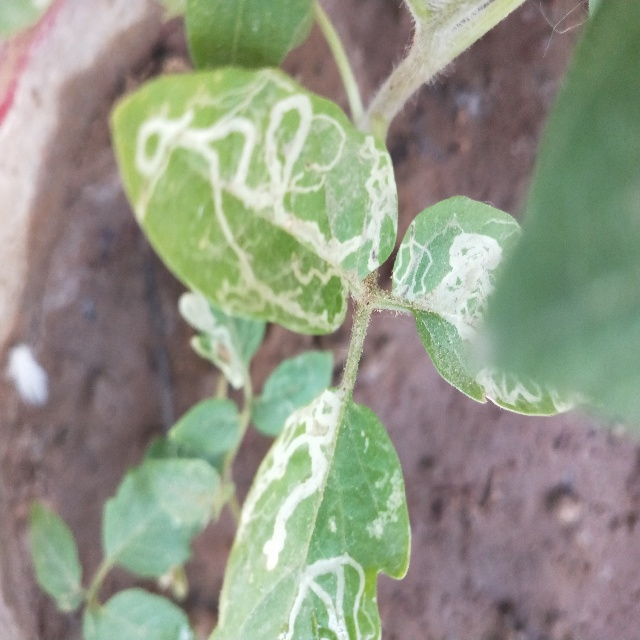
\includegraphics[width=3.2cm,height=3.2cm]{det_plant.png}};
\node[caplabel] at (-2.8,-3.0,0) {input plant, $640^2{\times}3$};

\pic at (0,0,0)
     {Box={name=st1,caption=Conv $3{\times}3$/2,%
       xlabel={{"64",""}},zlabel=$320^2$,fill=tStem,opacity=0.85,%
       height=44,width=18,depth=9}};
\pic[shift={(3.6,0,0)}] at (st1-east)
     {Box={name=st2,caption=Conv $3{\times}3$/2,%
       xlabel={{"128",""}},zlabel=$160^2$,fill=tStem,opacity=0.85,%
       height=34,width=20,depth=9}};
\pic[shift={(3.8,0,0)}] at (st2-east)
     {Box={name=s2,caption=TomaLayer$\times2$,%
       xlabel={{"128",""}},zlabel=$160^2$,fill=tTrunk,opacity=0.85,%
       height=34,width=22,depth=9}};
\pic[shift={(4.0,0,0)}] at (s2-east)
     {Box={name=s3,caption=TomaLayer$\times4$,%
       xlabel={{"256",""}},zlabel=$80^2$,fill=tTrunk,opacity=0.85,%
       height=24,width=24,depth=9}};
\pic[shift={(4.0,0,0)}] at (s3-east)
     {Box={name=s4,caption=TomaLayer$\times4$,%
       xlabel={{"512",""}},zlabel=$40^2$,fill=tTrunk,opacity=0.85,%
       height=16,width=26,depth=9}};
\pic[shift={(4.0,0,0)}] at (s4-east)
     {Box={name=s5,caption=TomaLayer$\times2$,%
       xlabel={{"1024",""}},zlabel=$20^2$,fill=tTrunk,opacity=0.85,%
       height=9,width=28,depth=8}};
\pic[shift={(3.4,0,0)}] at (s5-east)
     {Box={name=sppf,caption=SPPF $5{\times}5$,%
       xlabel={{"1024",""}},fill=tTrunk,opacity=0.7,%
       height=9,width=20,depth=8}};
\node[taglabel] at ($(s3-anchor)+(0,3.4,0)$) {$P3/8$ tap};
\node[taglabel] at ($(s4-anchor)+(0,2.6,0)$) {$P4/16$ tap};

\draw[connection] (input.east)  -- node{\midarrow} (st1-nearwest);
\draw[connection] (st1-neareast)-- node{\midarrow} (st2-nearwest);
\draw[connection] (st2-neareast)-- node{\midarrow} (s2-nearwest);
\draw[connection] (s2-neareast) -- node{\midarrow} (s3-nearwest);
\draw[connection] (s3-neareast) -- node{\midarrow} (s4-nearwest);
\draw[connection] (s4-neareast) -- node{\midarrow} (s5-nearwest);
\draw[connection] (s5-neareast) -- node{\midarrow} (sppf-nearwest);

% ----------------------------------------------------------------
% L1 (y=-11): top-down fusion at P4
% ----------------------------------------------------------------
\pic at ($(s4-anchor)+(0,-11,0)$)
     {Box={name=up4,caption=upsample $\times2$,%
       xlabel={{"nn",""}},fill=tStruct,opacity=0.9,height=16,width=14,depth=6}};
\pic[shift={(3.0,0,0)}] at (up4-east)
     {Ball={name=cat4,caption={concat $P4$},fill=tStruct,opacity=0.85,radius=2.0,logo={C}}};
\pic[shift={(2.6,0,0)}] at (cat4-east)
     {Box={name=n4,caption=TomaLayer$\times2$,%
       xlabel={{"512",""}},fill=tNeck,opacity=0.85,height=16,width=22,depth=9}};

\draw[connection] (sppf-south) -- ++(0,-2.2,0) -| (up4-north);
\draw[connection] (s4-south)   -- ++(0,-4.5,0) -| (cat4-north);
\draw[connection] (up4-neareast) -- node{\midarrow} (cat4-west);
\draw[connection] (cat4-east)  -- node{\midarrow} (n4-nearwest);

% ----------------------------------------------------------------
% L2 (y=-22): top-down fusion at P3 -- final small-object output
% ----------------------------------------------------------------
\pic at ($(s3-anchor)+(0,-22,0)$)
     {Box={name=up3,caption=upsample $\times2$,%
       xlabel={{"nn",""}},fill=tStruct,opacity=0.9,height=24,width=14,depth=6}};
\pic[shift={(3.0,0,0)}] at (up3-east)
     {Ball={name=cat3,caption={concat $P3$},fill=tStruct,opacity=0.85,radius=2.2,logo={C}}};
\pic[shift={(2.6,0,0)}] at (cat3-east)
     {Box={name=n3,caption=TomaLayer$\times2$,%
       xlabel={{"256",""}},fill=tNeck,opacity=0.85,height=24,width=20,depth=9}};
\node[taglabel] at ($(n3-south)+(0,-2.8,0)$) {$P3/8$ -- small};

\draw[connection] (n4-south) -- ++(0,-4.5,0) -| (up3-north);
\draw[connection] (s3-south) -- ++(0,-14.5,0) -| (cat3-north);
\draw[connection] (up3-neareast) -- node{\midarrow} (cat3-west);
\draw[connection] (cat3-east)-- node{\midarrow} (n3-nearwest);

\pic[shift={(3.2,0,0)}] at (n3-east)
     {Box={name=h3,caption=Detect head,%
       xlabel={{"box",""}},fill=tHeadD,opacity=0.85,height=15,width=16,depth=8}};
\draw[connection] (n3-neareast) -- node{\midarrow} (h3-nearwest);

% ----------------------------------------------------------------
% L3 (y=-33): bottom-up fusion at P4 -- final medium-object output
% ----------------------------------------------------------------
\pic at ($(n3-anchor)+(0,-11,0)$)
     {Box={name=dn3,caption=Conv $3{\times}3$/2,%
       xlabel={{"dn",""}},fill=tStem,opacity=0.85,height=16,width=14,depth=6}};
\pic[shift={(3.0,0,0)}] at (dn3-east)
     {Ball={name=cat4b,caption=concat,fill=tStruct,opacity=0.85,radius=2.0,logo={C}}};
\pic[shift={(2.6,0,0)}] at (cat4b-east)
     {Box={name=n4b,caption=TomaLayer$\times2$,%
       xlabel={{"512",""}},fill=tNeck,opacity=0.85,height=16,width=22,depth=9}};
\node[taglabel] at ($(n4b-south)+(0,-2.8,0)$) {$P4/16$ -- medium};

\draw[connection] (n3-south) |- (dn3-north);
\draw[skip] (n4-neareast) -- ++(1.4,0,0) -- ++(0,-22,0) -| (cat4b-north);
\draw[connection] (dn3-neareast) -- node{\midarrow} (cat4b-west);
\draw[connection] (cat4b-east)-- node{\midarrow} (n4b-nearwest);

\pic[shift={(3.2,0,0)}] at (n4b-east)
     {Box={name=h4,caption=Detect head,%
       xlabel={{"box",""}},fill=tHeadD,opacity=0.85,height=15,width=16,depth=8}};
\draw[connection] (n4b-neareast) -- node{\midarrow} (h4-nearwest);

% ----------------------------------------------------------------
% L4 (y=-44): bottom-up fusion at P5 -- final large-object output
% ----------------------------------------------------------------
\pic at ($(n4b-anchor)+(0,-11,0)$)
     {Box={name=dn4,caption=Conv $3{\times}3$/2,%
       xlabel={{"dn",""}},fill=tStem,opacity=0.85,height=9,width=14,depth=5}};
\pic[shift={(3.0,0,0)}] at (dn4-east)
     {Ball={name=cat5b,caption=concat,fill=tStruct,opacity=0.85,radius=1.8,logo={C}}};
\pic[shift={(2.6,0,0)}] at (cat5b-east)
     {Box={name=n5b,caption=TomaLayer$\times2$,%
       xlabel={{"1024",""}},fill=tNeck,opacity=0.85,height=9,width=24,depth=8}};
\node[taglabel] at ($(n5b-south)+(0,-2.8,0)$) {$P5/32$ -- large};

\draw[connection] (n4b-south) |- (dn4-north);
\draw[skip] (sppf-neareast) -- ++(24,0,0) -- ++(0,-44,0) -| (cat5b-north);
\draw[connection] (dn4-neareast) -- node{\midarrow} (cat5b-west);
\draw[connection] (cat5b-east)-- node{\midarrow} (n5b-nearwest);

\pic[shift={(3.2,0,0)}] at (n5b-east)
     {Box={name=h5,caption=Detect head,%
       xlabel={{"box",""}},fill=tHeadD,opacity=0.85,height=15,width=16,depth=8}};
\draw[connection] (n5b-neareast) -- node{\midarrow} (h5-nearwest);

% ----------------------------------------------------------------
% output: converge the 3 heads onto one prediction
% ----------------------------------------------------------------
\node[canvas is zy plane at x=0] (output) at ($(h4-east)+(4.0,0,0)$)
      {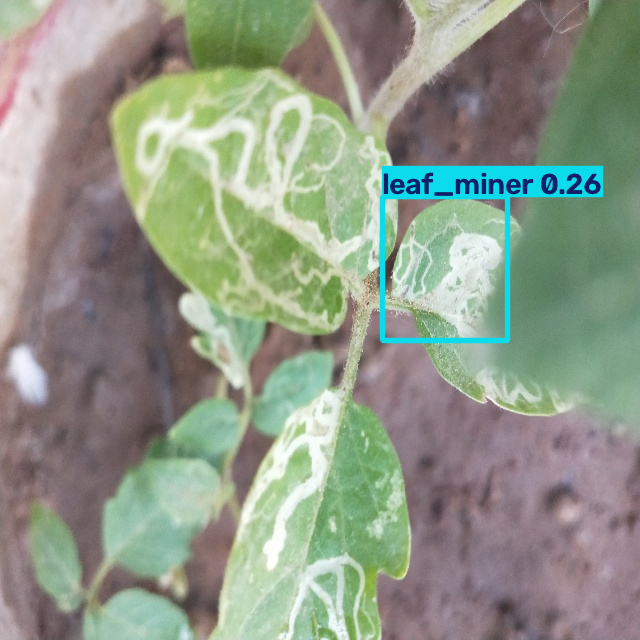
\includegraphics[width=3.4cm,height=3.4cm]{det_plant_pred.png}};
\node[caplabel] at ($(h4-east)+(4.0,-3.0,0)$)
      {\texttt{leaf\_miner}, $0.26$ (after NMS)};

\draw[connection] (h3-neareast) -- ++(1.4,0,0) |- (output.west);
\draw[connection] (h4-neareast) -- node{\midarrow} (output.west);
\draw[connection] (h5-neareast) -- ++(1.4,0,0) |- (output.west);

\end{tikzpicture}
\end{document}
